%%%%%%%%%%%%%%%%%%%%%%%%%%%%%%%%%%%%%%%%%
% Short Sectioned Assignment
% LaTeX Template
% Version 1.0 (5/5/12)
%
% This template has been downloaded from:
% http://www.LaTeXTemplates.com
%
% Original author:
% Frits Wenneker (http://www.howtotex.com)
%
% License:
% CC BY-NC-SA 3.0 (http://creativecommons.org/licenses/by-nc-sa/3.0/)
%
%%%%%%%%%%%%%%%%%%%%%%%%%%%%%%%%%%%%%%%%%

%----------------------------------------------------------------------------------------
%	PACKAGES AND OTHER DOCUMENT CONFIGURATIONS
%----------------------------------------------------------------------------------------

\documentclass[paper=a4, fontsize=11pt]{scrartcl} % A4 paper and 11pt font size

\usepackage[T1]{fontenc} % Use 8-bit encoding that has 256 glyphs
\usepackage{fourier} % Use the Adobe Utopia font for the document - comment this line to return to the LaTeX default
\usepackage[english]{babel} % English language/hyphenation
\usepackage{amsmath,amsfonts,amsthm} % Math packages
\usepackage{enumerate}
\usepackage{lipsum} % Used for inserting dummy 'Lorem ipsum' text into the template

\usepackage{sectsty} % Allows customizing section commands
\allsectionsfont{\centering \normalfont\scshape} % Make all sections centered, the default font and small caps
\sectionfont{\raggedright}
\usepackage[english]{babel}
\usepackage{mathtools}
\usepackage{graphicx}
\graphicspath{ {img/} }
\usepackage{pbox}


\usepackage{fancyhdr} % Custom headers and footers
\pagestyle{fancyplain} % Makes all pages in the document conform to the custom headers and footers
\fancyhead{} % No page header - if you want one, create it in the same way as the footers below
\fancyfoot[L]{} % Empty left footer
\fancyfoot[C]{} % Empty center footer
\fancyfoot[R]{\thepage} % Page numbering for right footer
\renewcommand{\headrulewidth}{0pt} % Remove header underlines
\renewcommand{\footrulewidth}{0pt} % Remove footer underlines
\setlength{\headheight}{13.6pt} % Customize the height of the header

\numberwithin{equation}{section} % Number equations within sections (i.e. 1.1, 1.2, 2.1, 2.2 instead of 1, 2, 3, 4)
\numberwithin{figure}{section} % Number figures within sections (i.e. 1.1, 1.2, 2.1, 2.2 instead of 1, 2, 3, 4)
\numberwithin{table}{section} % Number tables within sections (i.e. 1.1, 1.2, 2.1, 2.2 instead of 1, 2, 3, 4)

\setlength\parindent{0pt} % Removes all indentation from paragraphs - comment this line for an assignment with lots of text

%----------------------------------------------------------------------------------------
%	TITLE SECTION
%----------------------------------------------------------------------------------------

\newcommand{\horrule}[1]{\rule{\linewidth}{#1}} % Create horizontal rule command with 1 argument of height

\title{	
\normalfont \normalsize 
\textsc{National Taiwan University, \\ Graduate Institute of Biomedical Engineering and Bioinformatics} \\ [25pt] % Your university, school and/or department name(s)
\horrule{0.5pt} \\[0.4cm] % Thin top horizontal rule
\huge Mathematical Modeling of System Biology \\ Homework 1 \\ % The assignment title
\horrule{2pt} \\[0.5cm] % Thick bottom horizontal rule
}

\author{Yi Hsiao} % Your name

\date{\normalsize\today} % Today's date or a custom date
\begin{document}

\maketitle % Print the title

%----------------------------------------------------------------------------------------
%	PROBLEM 1
%----------------------------------------------------------------------------------------
\newpage
\section{}
Complete the following table. Assume mass action kinetics for all reaction mechanisms.

\begin{center}
    \begin{tabular}{| l | l | l | l |}
    \hline
    &Interaction graph&Rate equation scheme&ODE\\ \hline
	a) & $\xrightarrow{} A\xrightarrow{}$ & \raisebox{-\totalheight}{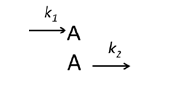
\includegraphics{1a}} & $\frac{d\left[A\right]}{dt}=k_{1}-k_{2}\left[A \right]$\\ \hline
    b) & \raisebox{-\totalheight}{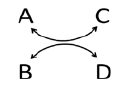
\includegraphics{1b}} & $A+B\xleftrightarrow[k_{-1}]{k_{1}}C+D$ & \parbox{5cm}{$\frac{d\left[A\right]}{dt}=-k_{1}\left[A \right]\left[B \right]+k_{-1}\left[C \right]\left[D \right]$,\\ $\frac{d\left[B\right]}{dt}=-k_{1}\left[A \right]\left[B \right]+k_{-1}\left[C \right]\left[D \right]$, \\ $\frac{d\left[C\right]}{dt}=k_{1}\left[A \right]\left[B \right]-k_{-1}\left[C \right]\left[D \right]$, \\ $\frac{d\left[D\right]}{dt}=k_{1}\left[A \right]\left[B \right]-k_{-1}\left[C \right]\left[D \right]$} \\ \hline
    c) & \raisebox{-\totalheight}{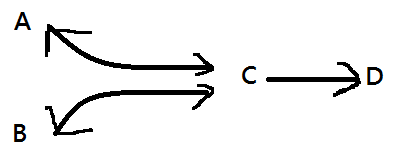
\includegraphics[scale=0.35]{1c-1}} & \parbox{5cm}{$A+B\xleftrightarrow[k_{-1}]{k_{1}}C\xrightarrow{k_{2}} D$} & \raisebox{-\totalheight}{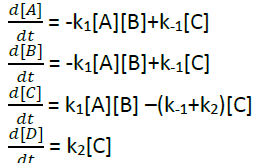
\includegraphics[scale=0.7]{1c}}  \\\hline
    d) & \raisebox{-\totalheight}{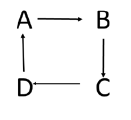
\includegraphics{1d}} & \parbox{5cm}{$A\xrightarrow{k_{1}}B$ \\ $B\xrightarrow{k_{2}}C$\\ $C\xrightarrow{k_{3}}D$ \\ $D\xrightarrow{k_{4}}A$ } & \parbox{5cm}{$\frac{d\left[A\right]}{dt}=-k_{1}\left[A \right]+k_{4}\left[D \right]$ \\ $\frac{d\left[B\right]}{dt}=-k_{2}\left[B \right]+k_{1}\left[A \right]$ \\ $\frac{d\left[C\right]}{dt}=-k_{3}\left[C \right]+k_{2}\left[B \right]$ \\ $\frac{d\left[D\right]}{dt}=-k_{4}\left[D \right]+k_{3}\left[C \right]$}  \\\hline
    e) & \raisebox{-\totalheight}{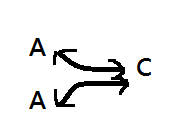
\includegraphics{1e-1}} & \raisebox{-\totalheight}{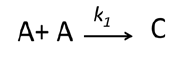
\includegraphics{1e}} & \parbox{5cm}{$\frac{d\left[A\right]}{dt}=-2k_{1}\left[A \right]^{2}$, \\ $\frac{d\left[C\right]}{dt}=k_{1}\left[A \right]^{2}$}\\\hline
    \end{tabular}
\end{center}

\section{}
\subsection{Problem Set 2.4.7}
\begin{enumerate}[a)]
	\item Consider the closed reaction network in Figure 2.16 with reaction rates $v_{i}$ as indicated. Suppose that the reaction rates are given by mass action as $v_{1}= k_{1}\left[ A \right]\left[ B \right]$, $v_{2} = k_{2}\left[ D \right]$ and $v_{3} = k_{3}\left[ C \right]$.
	\begin{enumerate}[i)]
	\item Construct a differential equation model for the network. Use moiety conservations to reduce your model to three differential equations and three algebraic equations.

	Initially, we can construct a set of differential equations of every species.
	\begin{align*}
		\frac{d\left[ A \right]}{dt}&=-v_{1},&\frac{d\left[ B \right]}{dt}&=-v_{1}+v_{2},&
		\frac{d\left[ C \right]}{dt}&=v_{1}-v_{3},&\\
		\frac{d\left[ D \right]}{dt}&=v_{1}-v_{2},&\frac{d\left[ E \right]}{dt}&=v_{3},&
		\frac{d\left[ F \right]}{dt}&=v_{3}\\
	\end{align*}
	Then, we can further combine many differential equation to make this set of equations smaller, because there are only three independent variables. Actually, we only need three linearly independent equations. That is, the three differential equations can be derived by moiety conservations: \\
	\begin{align*}
		\frac{d\left[ A \right]}{dt}+\frac{d\left[ C \right]}{dt}+\frac{d\left[ E \right]}{dt}&=0,&
		\frac{d\left[ A \right]}{dt}+\frac{d\left[ C \right]}{dt}+\frac{d\left[ F \right]}{dt}&=0,&
		\frac{d\left[ B \right]}{dt}+\frac{d\left[ D \right]}{dt}&=0,&
	\end{align*}
	where the three algebraic equations are
	\begin{align*}
		v_{1}&=k_{1}\left[ A \right]\left[ B \right],&v_{2}&=k_{2}\left[ D \right],&v_{3}&=k_{3}\left[ C \right]
	\end{align*}

	\item Solve for the steady-state concentrations as functions of the rate constants and the initial concentrations. (Note, because the system is closed, some of the steady-state concentrations are zero.)

	
	
	\item Verify your result in part (ii) by running a simulation of the system from initial conditions (in mM) of ([A], [B], [C], [D], [E], [F]) = (1, 1, 1 , 0, 0, 0). Take rate constants k1 = 3/mM/sec, k2 = 1/sec, k3 = 4/sec.
	\end{enumerate}
	\item Next consider the open system in Figure 2.17 with reaction rates vi as indicated. Suppose that the reaction rates are given by mass action as v0 = k0, v1 = k1[A][B], v2 = k2[D], v3 = k3[C], v4 = k4[E], and v5 = k5[F].
\end{enumerate}

\subsection{Problem Set 2.4.8}

\subsection{Problem Set 2.4.9}

%----------------------------------------------------------------------------------------

\end{document}